% =============================================================================
% PACER framework figure (self-contained TikZ; only requires \usepackage{tikz}
% in the main preamble). Components are grounded in the implementation:
%   - RT  : TRIER_RT reverse transformer, trained first, frozen during PT
%   - fuse: item + type(masked-mean category) + author + music + position
%   - PT  : forward transformer with dense per-position CE + cross-view NCE
%   - gen : step-wise top-k generation; greedy P_rel vs diverse
%           (1-lambda)P_rel + lambda P_cov paths (TRAINING paths shared by
%           L_div); NO lambda_c term here.
%   - sco : INFERENCE-only selection score S_s(j); this is the sole node that
%           carries the hard adjacent penalty -lambda_c C_s(j).
%   - losses: L_ce (dense), L_nce, L_div (ILD advantage),
%             gamma_o L_order (soft adjacent order, TRAINING only).
%   Routing rule: solid arrows = inference branch (sco -> R lists);
%   dashed arrows = training branch; the two never share an edge.
%
% LAYOUT NOTE: node minimum widths MUST be at least as wide as their longest
% text line. TikZ silently grows narrower nodes, sliding their west anchor
% left so neighbours overlap and arrows then point "backwards". If a box text
% changes, re-check its width (compile + render) before trusting the arrows.
%
% Input this file from approach.tex with % =============================================================================
% PACER framework figure (self-contained TikZ; only requires \usepackage{tikz}
% in the main preamble). Components are grounded in the implementation:
%   - RT  : TRIER_RT reverse transformer, trained first, frozen during PT
%   - fuse: item + type(masked-mean category) + author + music + position
%   - PT  : forward transformer with dense per-position CE + cross-view NCE
%   - gen : step-wise top-k generation; greedy P_rel vs diverse
%           (1-lambda)P_rel + lambda P_cov paths (TRAINING paths shared by
%           L_div); NO lambda_c term here.
%   - sco : INFERENCE-only selection score S_s(j); this is the sole node that
%           carries the hard adjacent penalty -lambda_c C_s(j).
%   - losses: L_ce (dense), L_nce, L_div (ILD advantage),
%             gamma_o L_order (soft adjacent order, TRAINING only).
%   Routing rule: solid arrows = inference branch (sco -> R lists);
%   dashed arrows = training branch; the two never share an edge.
%
% LAYOUT NOTE: node minimum widths MUST be at least as wide as their longest
% text line. TikZ silently grows narrower nodes, sliding their west anchor
% left so neighbours overlap and arrows then point "backwards". If a box text
% changes, re-check its width (compile + render) before trusting the arrows.
%
% Input this file from approach.tex with % =============================================================================
% PACER framework figure (self-contained TikZ; only requires \usepackage{tikz}
% in the main preamble). Components are grounded in the implementation:
%   - RT  : TRIER_RT reverse transformer, trained first, frozen during PT
%   - fuse: item + type(masked-mean category) + author + music + position
%   - PT  : forward transformer with dense per-position CE + cross-view NCE
%   - gen : step-wise top-k generation; greedy P_rel vs diverse
%           (1-lambda)P_rel + lambda P_cov paths (TRAINING paths shared by
%           L_div); NO lambda_c term here.
%   - sco : INFERENCE-only selection score S_s(j); this is the sole node that
%           carries the hard adjacent penalty -lambda_c C_s(j).
%   - losses: L_ce (dense), L_nce, L_div (ILD advantage),
%             gamma_o L_order (soft adjacent order, TRAINING only).
%   Routing rule: solid arrows = inference branch (sco -> R lists);
%   dashed arrows = training branch; the two never share an edge.
%
% LAYOUT NOTE: node minimum widths MUST be at least as wide as their longest
% text line. TikZ silently grows narrower nodes, sliding their west anchor
% left so neighbours overlap and arrows then point "backwards". If a box text
% changes, re-check its width (compile + render) before trusting the arrows.
%
% Input this file from approach.tex with % =============================================================================
% PACER framework figure (self-contained TikZ; only requires \usepackage{tikz}
% in the main preamble). Components are grounded in the implementation:
%   - RT  : TRIER_RT reverse transformer, trained first, frozen during PT
%   - fuse: item + type(masked-mean category) + author + music + position
%   - PT  : forward transformer with dense per-position CE + cross-view NCE
%   - gen : step-wise top-k generation; greedy P_rel vs diverse
%           (1-lambda)P_rel + lambda P_cov paths (TRAINING paths shared by
%           L_div); NO lambda_c term here.
%   - sco : INFERENCE-only selection score S_s(j); this is the sole node that
%           carries the hard adjacent penalty -lambda_c C_s(j).
%   - losses: L_ce (dense), L_nce, L_div (ILD advantage),
%             gamma_o L_order (soft adjacent order, TRAINING only).
%   Routing rule: solid arrows = inference branch (sco -> R lists);
%   dashed arrows = training branch; the two never share an edge.
%
% LAYOUT NOTE: node minimum widths MUST be at least as wide as their longest
% text line. TikZ silently grows narrower nodes, sliding their west anchor
% left so neighbours overlap and arrows then point "backwards". If a box text
% changes, re-check its width (compile + render) before trusting the arrows.
%
% Input this file from approach.tex with \input{figures/pacer_framework.tex}.
% =============================================================================
\usetikzlibrary{arrows.meta,positioning,fit,backgrounds}

% Float placement notes (two-column):
%  - [t!] overrides LaTeX's aesthetic limits so the spanning float can take
%    the top of the *next* page even when tall.
%  - Preamble (main .tex), recommended:
%      \usepackage{dblfloatfix}                 % allow current-page placement
%      \usepackage{placeins}                    % \FloatBarrier support
%      \renewcommand{\dbltopfraction}{0.95}
%      \renewcommand{\dblfloatpagefraction}{0.7}
%  - To stop it drifting past a section, put \FloatBarrier where it must be
%    printed by (e.g. right before the next \subsection).
%  - Exact "on this page, right here" needs a non-float: use the strip
%    environment of the cuted package instead of figure*.
\begin{figure*}[t!]
\centering
% Overall size knob: fraction of the (two-column-spanning) \textwidth.
%   1.0\textwidth = full span (current); 0.8/0.7 = smaller, auto-centred.
% For a one-column figure: change figure* -> figure and use \columnwidth here.
% Prefer 0.85-1.0: below ~0.7 the scaled math/labels get hard to read; in that
% case shrink internals instead (font=\footnotesize, smaller node dimensions).
\resizebox{0.9\textwidth}{!}{%
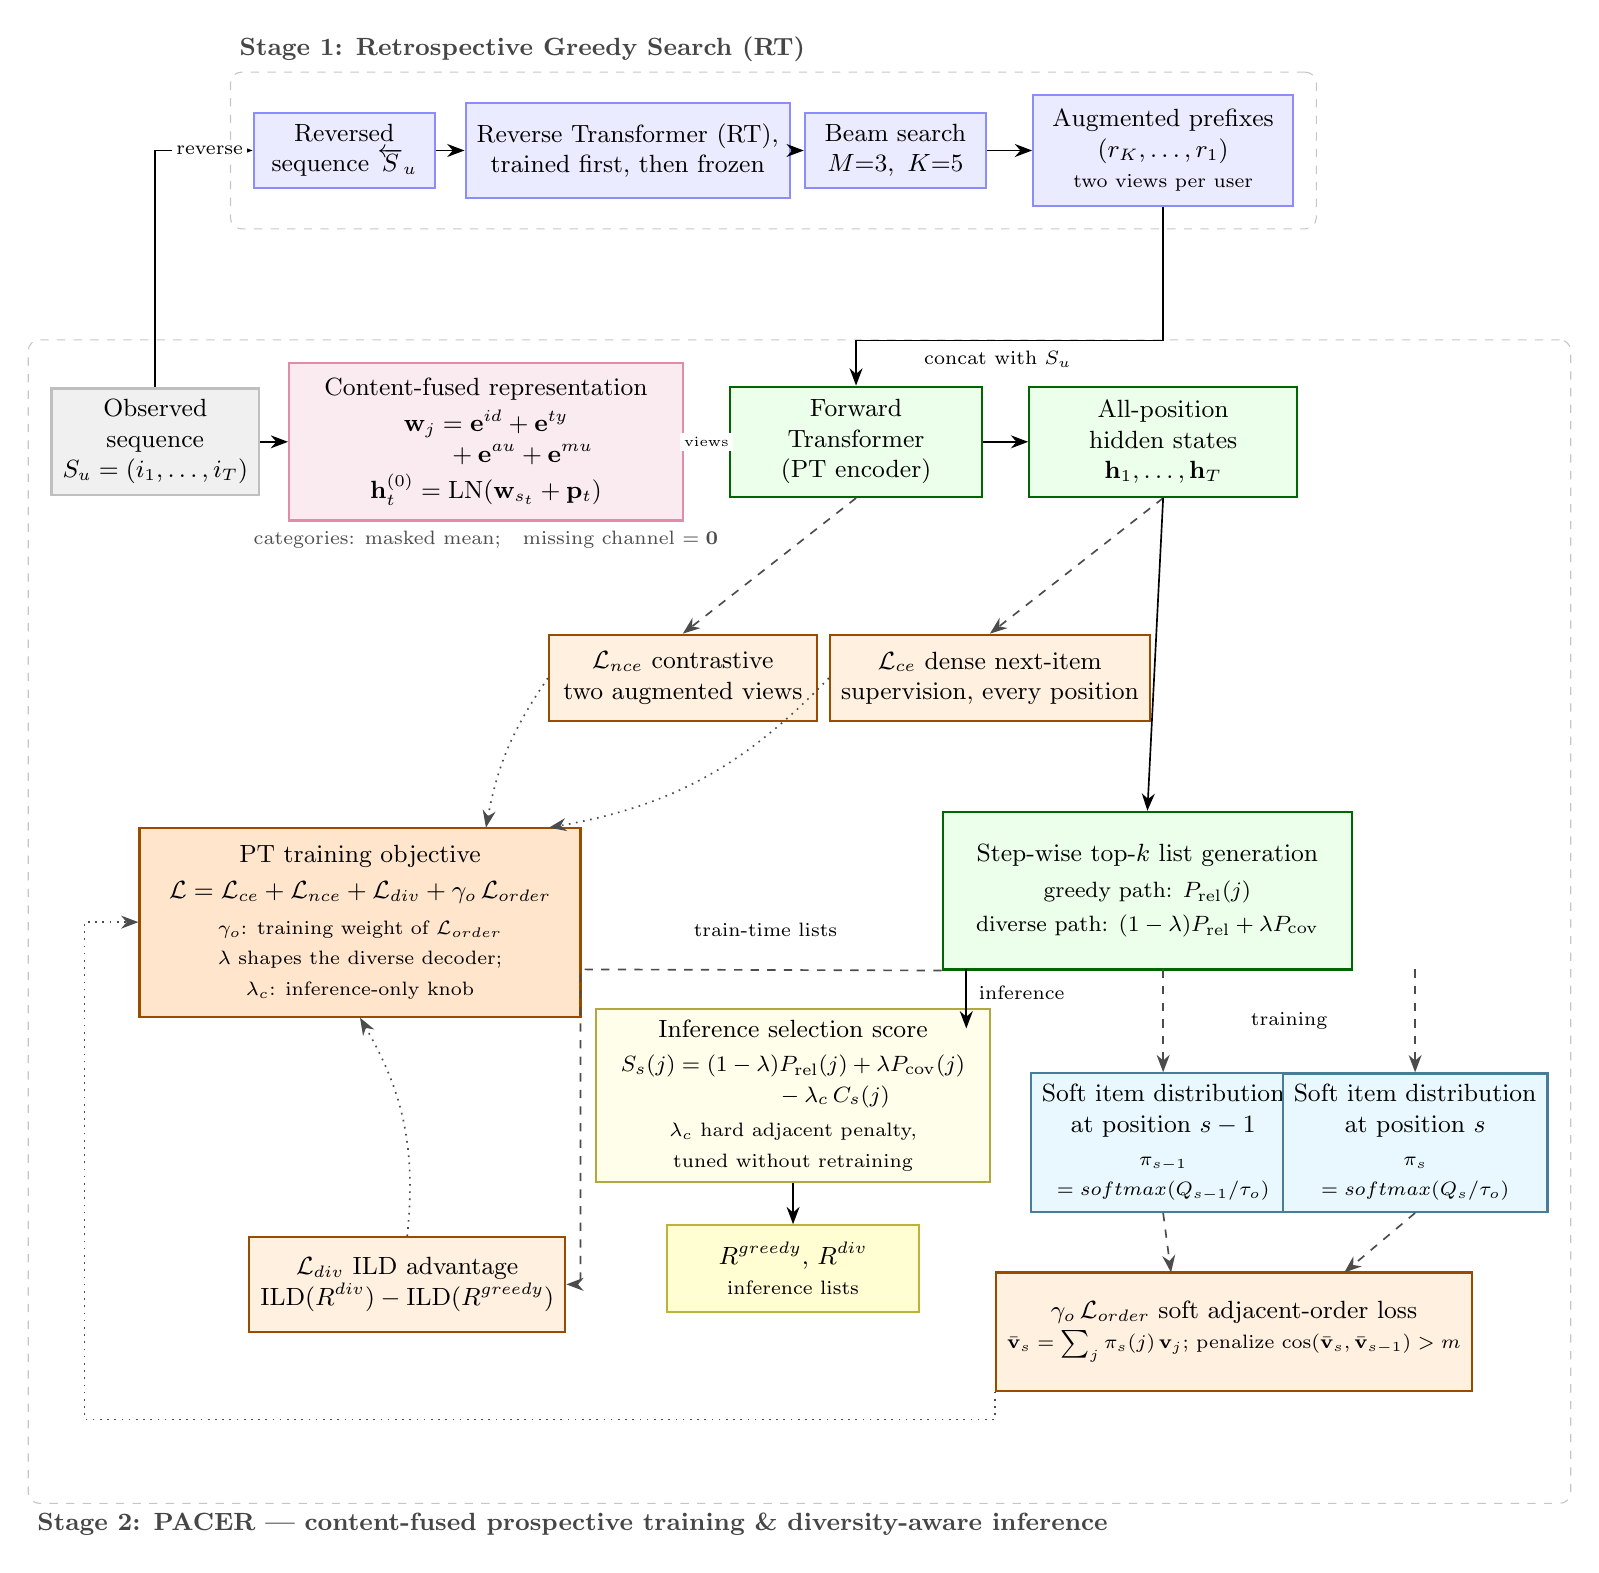
\begin{tikzpicture}[
  font=\small,
  box/.style={draw, align=center, inner sep=4pt,
              minimum height=0.95cm, thick},
  data/.style={box, fill=gray!12, draw=gray!50},
  rtb/.style={box, fill=blue!8, draw=blue!45},
  ptb/.style={box, fill=green!8, draw=green!40!black},
  emb/.style={box, fill=purple!8, draw=purple!45},
  loss/.style={box, fill=orange!12, draw=orange!60!black},
  softd/.style={box, fill=cyan!9, draw=cyan!55!black},
  lst/.style={box, fill=yellow!18, draw=yellow!70!black},
  scb/.style={box, fill=yellow!8, draw=yellow!65!black},
  arr/.style={-{Stealth[length=2.2mm]}, semithick},
  darr/.style={arr, dashed, gray!60!black},
  lbl/.style={font=\scriptsize, fill=white, inner sep=1.5pt},
  note/.style={font=\scriptsize, text=gray!60!black, align=center},
  stage/.style={draw=gray!45, dashed, rounded corners=4pt, inner sep=8pt},
  stagelbl/.style={font=\small\bfseries, text=gray!55!black}
]

% ---------------- main forward pipeline (y = 3.5) ----------------
\node[data, minimum width=2.6cm] (seq) at (0,3.5)
  {Observed\\ sequence\\ $S_u=(i_1,\ldots,i_T)$};

\node[emb, minimum width=5.0cm, minimum height=2.0cm] (fuse) at (4.2,3.5)
  {Content-fused representation\\[2pt]
   $\mathbf w_j=\mathbf e^{id}+\mathbf e^{ty}$\\
   $\phantom{\mathbf w_j=}\ +\mathbf e^{au}+\mathbf e^{mu}$\\[1pt]
   $\mathbf h_t^{(0)}=\mathrm{LN}(\mathbf w_{s_t}+\mathbf p_t)$};
\node[note, anchor=north] (fusenote) at (fuse.south)
  {categories: masked mean;\quad missing channel $=\mathbf 0$};

\node[ptb, minimum width=3.2cm, minimum height=1.4cm] (pte) at (8.9,3.5)
  {Forward\\ Transformer\\ (PT encoder)};

\node[ptb, minimum width=3.4cm, minimum height=1.4cm] (hs) at (12.8,3.5)
  {All-position\\ hidden states\\ $\mathbf h_1,\ldots,\mathbf h_T$};

\draw[arr] (seq.east) -- (fuse.west);
\draw[arr] (fuse.east) -- node[lbl, font=\tiny]{views} (pte.west);
\draw[arr] (pte.east) -- (hs.west);

% ---------------- Stage 1: RT (y = 7.2) ----------------
\node[rtb, minimum width=2.3cm] (rev) at (2.4,7.2)
  {Reversed\\ sequence $\overleftarrow S_u$};
\node[rtb, minimum width=3.2cm, minimum height=1.2cm] (rte) at (6.0,7.2)
  {Reverse Transformer (RT),\\ trained first, then frozen};
\node[rtb, minimum width=2.3cm] (beam) at (9.4,7.2)
  {Beam search\\ $M{=}3,\ K{=}5$};
\node[rtb, minimum width=3.3cm, minimum height=1.4cm] (pref) at (12.8,7.2)
  {Augmented prefixes\\ $(r_K,\ldots,r_1)$\\ {\scriptsize two views per user}};

\draw[arr] (seq.north) |- node[lbl, pos=0.78]{reverse} (rev.west);
\draw[arr] (rev.east) -- (rte.west);
\draw[arr] (rte.east) -- (beam.west);
\draw[arr] (beam.east) -- (pref.west);
% Route around the hidden-states box: down into the inter-row gap, then left,
% then into the top of the PT encoder.
\draw[arr] (pref.south) -- ++(0,-1.7) -| (pte.north);
\node[lbl] at (10.7,4.55) {concat with $S_u$};

% ---------------- training losses (y = 0.5) ----------------
\node[loss, minimum width=3.4cm, minimum height=1.1cm] (lnce) at (6.7,0.5)
  {$\mathcal L_{nce}$ contrastive\\ two augmented views};
\node[loss, minimum width=3.4cm, minimum height=1.1cm] (lce) at (10.6,0.5)
  {$\mathcal L_{ce}$ dense next-item\\ supervision, every position};
\draw[darr] (pte.south) -- (lnce.north);
\draw[darr] (hs.south) -- (lce.north);

% ---------------- total objective (bottom left) ----------------
\node[loss, fill=orange!20, minimum width=5.6cm, minimum height=2.4cm] (ltot)
  at (2.6,-2.6)
  {PT training objective\\[2pt]
   $\mathcal L=\mathcal L_{ce}+\mathcal L_{nce}+\mathcal L_{div}
    +\gamma_o\,\mathcal L_{order}$\\[2pt]
   {\scriptsize $\gamma_o$: training weight of $\mathcal L_{order}$}\\
   {\scriptsize $\lambda$ shapes the diverse decoder;}\\
   {\scriptsize $\lambda_c$: inference-only knob}};
% Both per-step losses feed the objective across its TOP edge, at distinct
% points, keeping the thin corridor UNDER the box (y=-3.2) completely clear.
\draw[darr, dotted] (lnce.west) to[bend right=12] (4.2,-1.4);
\draw[darr, dotted] (lce.west)  to[bend left=18]  (5.0,-1.4);

% ---------------- step-wise generation (right, y = -2.2) ----------------
% TRAINING-time generation: relevance path + diversity coverage path only.
% The hard adjacent penalty -lambda_c C_s(j) does NOT live here; it is applied
% exclusively in the inference selection-score node on the solid branch.
\node[ptb, minimum width=5.2cm, minimum height=2.0cm] (gen) at (12.6,-2.2)
  {Step-wise top-$k$ list generation\\[2pt]
   {\footnotesize greedy path: $P_{\mathrm{rel}}(j)$}\\[1pt]
   {\footnotesize diverse path:
    $(1-\lambda)P_{\mathrm{rel}}+\lambda P_{\mathrm{cov}}$}};
\draw[arr] (hs.south) -- (gen.north);

% ---------------- INFERENCE branch (SOLID): score then lists ---------------
% The FULL selection score, including -lambda_c C_s(j), exists only here.
\node[scb, minimum width=5.0cm, minimum height=1.7cm] (sco) at (8.1,-4.8)
  {Inference selection score\\[1.5pt]
   {\footnotesize $S_s(j)=(1-\lambda)P_{\mathrm{rel}}(j)
                       +\lambda P_{\mathrm{cov}}(j)$}\\
   {\footnotesize $\phantom{S_s(j)=}-\lambda_c\,C_s(j)$}\\[1.5pt]
   {\scriptsize $\lambda_c$ hard adjacent penalty,}\\
   {\scriptsize tuned without retraining}};
% Pure deployment output: this node has NO arrows into training losses.
\node[lst, minimum width=3.2cm, minimum height=1.1cm] (ri) at (8.1,-7.0)
  {$R^{greedy},\,R^{div}$\\ {\scriptsize inference lists}};
% Solid inference branch leaves gen just inside its SW corner and drops into
% the score node's north edge (short, entirely to the right of the score box).
\draw[arr] (10.3,-3.2) -- (10.3,-3.95);
\node[lbl, anchor=west] at (10.4,-3.5) {inference};
\draw[arr] (sco.south) -- (ri.north);

% ---------------- training-time soft distributions (DASHED branch) ----------
% The decoder scores Q_s at two adjacent positions are turned into soft item
% distributions; L_order reads BOTH of them (never an argmax'd token).
\node[softd, minimum width=3.0cm, minimum height=1.5cm] (pip) at (12.8,-5.4)
  {Soft item distribution\\ at position $s-1$\\[1pt]
   {\scriptsize $\boldsymbol\pi_{s-1}$}\\
   {\scriptsize $=\operatorname{softmax}(Q_{s-1}/\tau_o)$}};
\node[softd, minimum width=3.0cm, minimum height=1.5cm] (pi) at (16.0,-5.4)
  {Soft item distribution\\ at position $s$\\[1pt]
   {\scriptsize $\boldsymbol\pi_s$}\\
   {\scriptsize $=\operatorname{softmax}(Q_s/\tau_o)$}};
\draw[darr] (12.8,-3.2) -- (pip.north);
\draw[darr] (16.0,-3.2) -- (pi.north);
\node[lbl] at (14.4,-3.85) {training};

% ---------------- list-level training losses (bottom row) ------------------
\node[loss, minimum width=4.0cm, minimum height=1.2cm] (ldiv) at (3.2,-7.2)
  {$\mathcal L_{div}$ ILD advantage\\
   $\mathrm{ILD}(R^{div})-\mathrm{ILD}(R^{greedy})$};
\node[loss, minimum width=4.4cm, minimum height=1.5cm] (lo) at (13.7,-7.8)
  {$\gamma_o\,\mathcal L_{order}$ soft adjacent-order loss\\
   {\scriptsize $\bar{\mathbf v}_s=\sum_j \pi_s(j)\,\mathbf v_j$;
    penalize $\cos(\bar{\mathbf v}_s,\bar{\mathbf v}_{s-1})>m$}};

% Train-time list comparison: dashed, leaves the gen SW corner (the solid
% inference arrow leaves 0.3cm to its right), runs west through the clear
% corridor between objective (south -3.8) and score (north -3.95), drops in
% the gap between them, and enters L_div from the east.
\draw[darr] (gen.south west) -- (5.4,-3.2) -- (5.4,-7.2) -- (ldiv.east);
\node[lbl, anchor=north] at (7.75,-2.55) {train-time lists};

% The TWO ADJACENT SOFT DISTRIBUTIONS both point to L_order.
\draw[darr] (pip.south) -- (12.9,-7.05);
\draw[darr] (pi.south)  -- (15.1,-7.05);

% Losses roll up into the total training objective. L_div -> objective is a
% short curve on the left; L_order leaves from its SW corner along the BOTTOM
% corridor (below the inference lists and every loss box), rises in the
% far-left gap and enters the objective from the west.
\draw[darr, dotted] (ldiv.north) to[bend right=18] (ltot.south);
\draw[darr, dotted] (lo.south west) -- ++(0,-0.35) -| (-0.9,-2.6)
  -- (ltot.west);

% ---------------- stage frames ----------------
% pads keep the bottom/left L_order -> objective connector inside the frame.
\coordinate (framepad) at (8.5,-9.7);
\coordinate (framepadl) at (-1.1,-2.6);
\begin{scope}[on background layer]
  \node[stage, fit=(rev)(rte)(beam)(pref)] (st1) {};
  \node[stage, fit=(seq)(fuse)(fusenote)(pte)(hs)(lnce)(lce)(gen)
                       (sco)(ri)(pip)(pi)(ldiv)(lo)(ltot)
                       (framepad)(framepadl)] (st2) {};
\end{scope}
\node[stagelbl, anchor=south west] at (st1.north west)
  {Stage 1: Retrospective Greedy Search (RT)};
\node[stagelbl, anchor=north west] at (st2.south west)
  {Stage 2: PACER --- content-fused prospective training \& diversity-aware inference};

\end{tikzpicture}%
}
\caption{Overall PACER framework. \textbf{Stage 1 (RT):} a reverse-direction
transformer, trained independently and then frozen, hallucinates items that
could have preceded the observed sequence and returns beam-search augmented
views. \textbf{Stage 2 (PACER):} each item is represented by additive fusion of
ID, category (masked-mean pooled), creator, and music embeddings together with
a positional embedding; a forward transformer is trained with dense
per-position next-item supervision ($\mathcal L_{ce}$), cross-view contrastive
learning ($\mathcal L_{nce}$), an ILD list-diversity loss
($\mathcal L_{div}$), and a differentiable \emph{soft} adjacent-order loss
($\gamma_o\mathcal L_{order}$) computed from the soft item distributions at two
neighbouring list positions rather than from argmax tokens (solid arrows mark
the inference branch, dashed arrows the training branch). At inference, lists
are generated step by step with the combined relevance--coverage score that
additionally carries the hard adjacent-content penalty $-\lambda_c C_s(j)$;
$\lambda_c$ is tuned without retraining.}
\label{fig:pacer_framework}
\end{figure*}
.
% =============================================================================
\usetikzlibrary{arrows.meta,positioning,fit,backgrounds}

% Float placement notes (two-column):
%  - [t!] overrides LaTeX's aesthetic limits so the spanning float can take
%    the top of the *next* page even when tall.
%  - Preamble (main .tex), recommended:
%      \usepackage{dblfloatfix}                 % allow current-page placement
%      \usepackage{placeins}                    % \FloatBarrier support
%      \renewcommand{\dbltopfraction}{0.95}
%      \renewcommand{\dblfloatpagefraction}{0.7}
%  - To stop it drifting past a section, put \FloatBarrier where it must be
%    printed by (e.g. right before the next \subsection).
%  - Exact "on this page, right here" needs a non-float: use the strip
%    environment of the cuted package instead of figure*.
\begin{figure*}[t!]
\centering
% Overall size knob: fraction of the (two-column-spanning) \textwidth.
%   1.0\textwidth = full span (current); 0.8/0.7 = smaller, auto-centred.
% For a one-column figure: change figure* -> figure and use \columnwidth here.
% Prefer 0.85-1.0: below ~0.7 the scaled math/labels get hard to read; in that
% case shrink internals instead (font=\footnotesize, smaller node dimensions).
\resizebox{0.9\textwidth}{!}{%
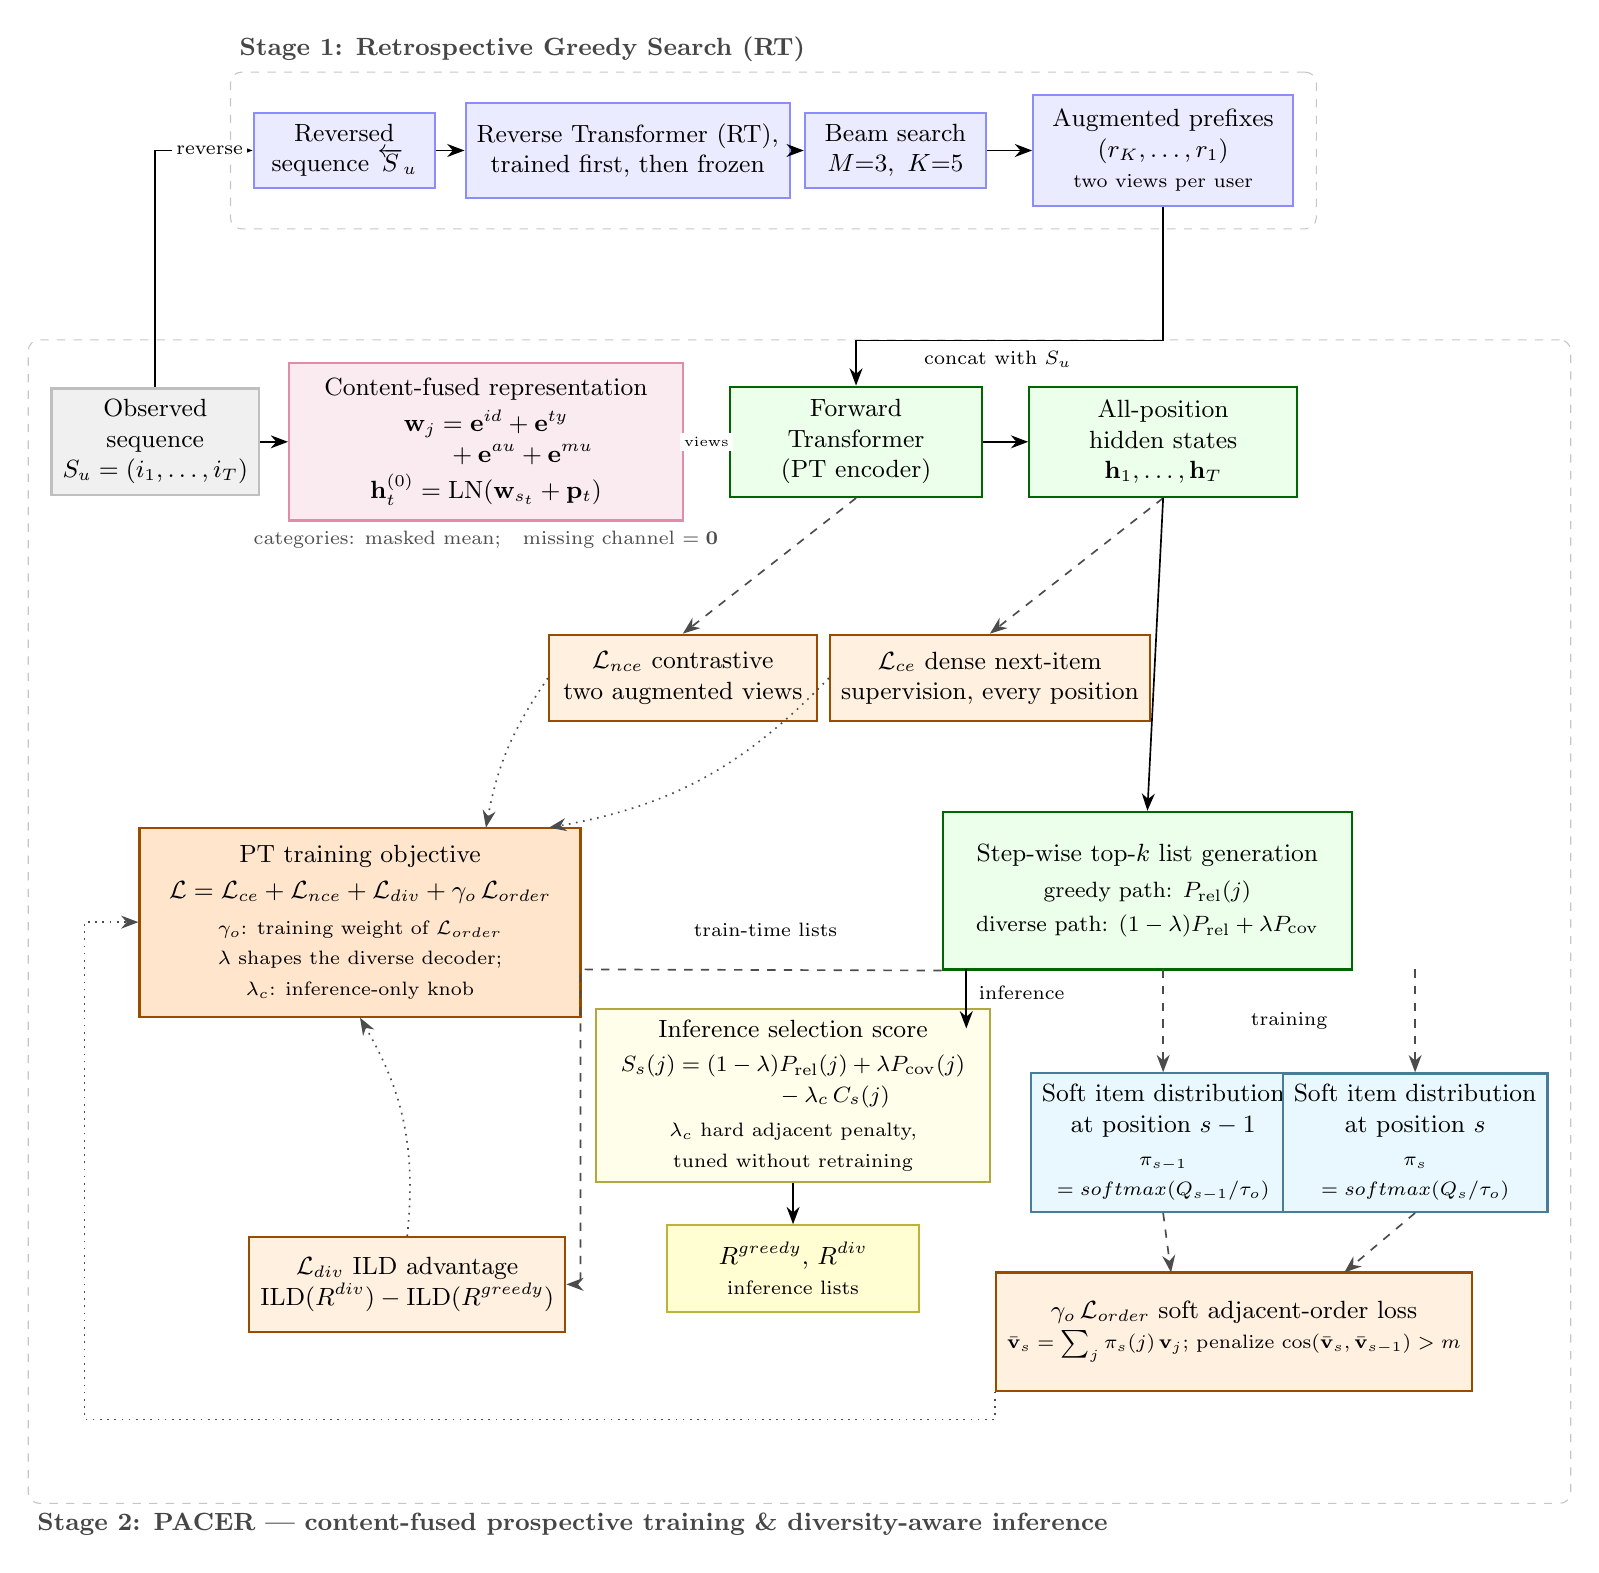
\begin{tikzpicture}[
  font=\small,
  box/.style={draw, align=center, inner sep=4pt,
              minimum height=0.95cm, thick},
  data/.style={box, fill=gray!12, draw=gray!50},
  rtb/.style={box, fill=blue!8, draw=blue!45},
  ptb/.style={box, fill=green!8, draw=green!40!black},
  emb/.style={box, fill=purple!8, draw=purple!45},
  loss/.style={box, fill=orange!12, draw=orange!60!black},
  softd/.style={box, fill=cyan!9, draw=cyan!55!black},
  lst/.style={box, fill=yellow!18, draw=yellow!70!black},
  scb/.style={box, fill=yellow!8, draw=yellow!65!black},
  arr/.style={-{Stealth[length=2.2mm]}, semithick},
  darr/.style={arr, dashed, gray!60!black},
  lbl/.style={font=\scriptsize, fill=white, inner sep=1.5pt},
  note/.style={font=\scriptsize, text=gray!60!black, align=center},
  stage/.style={draw=gray!45, dashed, rounded corners=4pt, inner sep=8pt},
  stagelbl/.style={font=\small\bfseries, text=gray!55!black}
]

% ---------------- main forward pipeline (y = 3.5) ----------------
\node[data, minimum width=2.6cm] (seq) at (0,3.5)
  {Observed\\ sequence\\ $S_u=(i_1,\ldots,i_T)$};

\node[emb, minimum width=5.0cm, minimum height=2.0cm] (fuse) at (4.2,3.5)
  {Content-fused representation\\[2pt]
   $\mathbf w_j=\mathbf e^{id}+\mathbf e^{ty}$\\
   $\phantom{\mathbf w_j=}\ +\mathbf e^{au}+\mathbf e^{mu}$\\[1pt]
   $\mathbf h_t^{(0)}=\mathrm{LN}(\mathbf w_{s_t}+\mathbf p_t)$};
\node[note, anchor=north] (fusenote) at (fuse.south)
  {categories: masked mean;\quad missing channel $=\mathbf 0$};

\node[ptb, minimum width=3.2cm, minimum height=1.4cm] (pte) at (8.9,3.5)
  {Forward\\ Transformer\\ (PT encoder)};

\node[ptb, minimum width=3.4cm, minimum height=1.4cm] (hs) at (12.8,3.5)
  {All-position\\ hidden states\\ $\mathbf h_1,\ldots,\mathbf h_T$};

\draw[arr] (seq.east) -- (fuse.west);
\draw[arr] (fuse.east) -- node[lbl, font=\tiny]{views} (pte.west);
\draw[arr] (pte.east) -- (hs.west);

% ---------------- Stage 1: RT (y = 7.2) ----------------
\node[rtb, minimum width=2.3cm] (rev) at (2.4,7.2)
  {Reversed\\ sequence $\overleftarrow S_u$};
\node[rtb, minimum width=3.2cm, minimum height=1.2cm] (rte) at (6.0,7.2)
  {Reverse Transformer (RT),\\ trained first, then frozen};
\node[rtb, minimum width=2.3cm] (beam) at (9.4,7.2)
  {Beam search\\ $M{=}3,\ K{=}5$};
\node[rtb, minimum width=3.3cm, minimum height=1.4cm] (pref) at (12.8,7.2)
  {Augmented prefixes\\ $(r_K,\ldots,r_1)$\\ {\scriptsize two views per user}};

\draw[arr] (seq.north) |- node[lbl, pos=0.78]{reverse} (rev.west);
\draw[arr] (rev.east) -- (rte.west);
\draw[arr] (rte.east) -- (beam.west);
\draw[arr] (beam.east) -- (pref.west);
% Route around the hidden-states box: down into the inter-row gap, then left,
% then into the top of the PT encoder.
\draw[arr] (pref.south) -- ++(0,-1.7) -| (pte.north);
\node[lbl] at (10.7,4.55) {concat with $S_u$};

% ---------------- training losses (y = 0.5) ----------------
\node[loss, minimum width=3.4cm, minimum height=1.1cm] (lnce) at (6.7,0.5)
  {$\mathcal L_{nce}$ contrastive\\ two augmented views};
\node[loss, minimum width=3.4cm, minimum height=1.1cm] (lce) at (10.6,0.5)
  {$\mathcal L_{ce}$ dense next-item\\ supervision, every position};
\draw[darr] (pte.south) -- (lnce.north);
\draw[darr] (hs.south) -- (lce.north);

% ---------------- total objective (bottom left) ----------------
\node[loss, fill=orange!20, minimum width=5.6cm, minimum height=2.4cm] (ltot)
  at (2.6,-2.6)
  {PT training objective\\[2pt]
   $\mathcal L=\mathcal L_{ce}+\mathcal L_{nce}+\mathcal L_{div}
    +\gamma_o\,\mathcal L_{order}$\\[2pt]
   {\scriptsize $\gamma_o$: training weight of $\mathcal L_{order}$}\\
   {\scriptsize $\lambda$ shapes the diverse decoder;}\\
   {\scriptsize $\lambda_c$: inference-only knob}};
% Both per-step losses feed the objective across its TOP edge, at distinct
% points, keeping the thin corridor UNDER the box (y=-3.2) completely clear.
\draw[darr, dotted] (lnce.west) to[bend right=12] (4.2,-1.4);
\draw[darr, dotted] (lce.west)  to[bend left=18]  (5.0,-1.4);

% ---------------- step-wise generation (right, y = -2.2) ----------------
% TRAINING-time generation: relevance path + diversity coverage path only.
% The hard adjacent penalty -lambda_c C_s(j) does NOT live here; it is applied
% exclusively in the inference selection-score node on the solid branch.
\node[ptb, minimum width=5.2cm, minimum height=2.0cm] (gen) at (12.6,-2.2)
  {Step-wise top-$k$ list generation\\[2pt]
   {\footnotesize greedy path: $P_{\mathrm{rel}}(j)$}\\[1pt]
   {\footnotesize diverse path:
    $(1-\lambda)P_{\mathrm{rel}}+\lambda P_{\mathrm{cov}}$}};
\draw[arr] (hs.south) -- (gen.north);

% ---------------- INFERENCE branch (SOLID): score then lists ---------------
% The FULL selection score, including -lambda_c C_s(j), exists only here.
\node[scb, minimum width=5.0cm, minimum height=1.7cm] (sco) at (8.1,-4.8)
  {Inference selection score\\[1.5pt]
   {\footnotesize $S_s(j)=(1-\lambda)P_{\mathrm{rel}}(j)
                       +\lambda P_{\mathrm{cov}}(j)$}\\
   {\footnotesize $\phantom{S_s(j)=}-\lambda_c\,C_s(j)$}\\[1.5pt]
   {\scriptsize $\lambda_c$ hard adjacent penalty,}\\
   {\scriptsize tuned without retraining}};
% Pure deployment output: this node has NO arrows into training losses.
\node[lst, minimum width=3.2cm, minimum height=1.1cm] (ri) at (8.1,-7.0)
  {$R^{greedy},\,R^{div}$\\ {\scriptsize inference lists}};
% Solid inference branch leaves gen just inside its SW corner and drops into
% the score node's north edge (short, entirely to the right of the score box).
\draw[arr] (10.3,-3.2) -- (10.3,-3.95);
\node[lbl, anchor=west] at (10.4,-3.5) {inference};
\draw[arr] (sco.south) -- (ri.north);

% ---------------- training-time soft distributions (DASHED branch) ----------
% The decoder scores Q_s at two adjacent positions are turned into soft item
% distributions; L_order reads BOTH of them (never an argmax'd token).
\node[softd, minimum width=3.0cm, minimum height=1.5cm] (pip) at (12.8,-5.4)
  {Soft item distribution\\ at position $s-1$\\[1pt]
   {\scriptsize $\boldsymbol\pi_{s-1}$}\\
   {\scriptsize $=\operatorname{softmax}(Q_{s-1}/\tau_o)$}};
\node[softd, minimum width=3.0cm, minimum height=1.5cm] (pi) at (16.0,-5.4)
  {Soft item distribution\\ at position $s$\\[1pt]
   {\scriptsize $\boldsymbol\pi_s$}\\
   {\scriptsize $=\operatorname{softmax}(Q_s/\tau_o)$}};
\draw[darr] (12.8,-3.2) -- (pip.north);
\draw[darr] (16.0,-3.2) -- (pi.north);
\node[lbl] at (14.4,-3.85) {training};

% ---------------- list-level training losses (bottom row) ------------------
\node[loss, minimum width=4.0cm, minimum height=1.2cm] (ldiv) at (3.2,-7.2)
  {$\mathcal L_{div}$ ILD advantage\\
   $\mathrm{ILD}(R^{div})-\mathrm{ILD}(R^{greedy})$};
\node[loss, minimum width=4.4cm, minimum height=1.5cm] (lo) at (13.7,-7.8)
  {$\gamma_o\,\mathcal L_{order}$ soft adjacent-order loss\\
   {\scriptsize $\bar{\mathbf v}_s=\sum_j \pi_s(j)\,\mathbf v_j$;
    penalize $\cos(\bar{\mathbf v}_s,\bar{\mathbf v}_{s-1})>m$}};

% Train-time list comparison: dashed, leaves the gen SW corner (the solid
% inference arrow leaves 0.3cm to its right), runs west through the clear
% corridor between objective (south -3.8) and score (north -3.95), drops in
% the gap between them, and enters L_div from the east.
\draw[darr] (gen.south west) -- (5.4,-3.2) -- (5.4,-7.2) -- (ldiv.east);
\node[lbl, anchor=north] at (7.75,-2.55) {train-time lists};

% The TWO ADJACENT SOFT DISTRIBUTIONS both point to L_order.
\draw[darr] (pip.south) -- (12.9,-7.05);
\draw[darr] (pi.south)  -- (15.1,-7.05);

% Losses roll up into the total training objective. L_div -> objective is a
% short curve on the left; L_order leaves from its SW corner along the BOTTOM
% corridor (below the inference lists and every loss box), rises in the
% far-left gap and enters the objective from the west.
\draw[darr, dotted] (ldiv.north) to[bend right=18] (ltot.south);
\draw[darr, dotted] (lo.south west) -- ++(0,-0.35) -| (-0.9,-2.6)
  -- (ltot.west);

% ---------------- stage frames ----------------
% pads keep the bottom/left L_order -> objective connector inside the frame.
\coordinate (framepad) at (8.5,-9.7);
\coordinate (framepadl) at (-1.1,-2.6);
\begin{scope}[on background layer]
  \node[stage, fit=(rev)(rte)(beam)(pref)] (st1) {};
  \node[stage, fit=(seq)(fuse)(fusenote)(pte)(hs)(lnce)(lce)(gen)
                       (sco)(ri)(pip)(pi)(ldiv)(lo)(ltot)
                       (framepad)(framepadl)] (st2) {};
\end{scope}
\node[stagelbl, anchor=south west] at (st1.north west)
  {Stage 1: Retrospective Greedy Search (RT)};
\node[stagelbl, anchor=north west] at (st2.south west)
  {Stage 2: PACER --- content-fused prospective training \& diversity-aware inference};

\end{tikzpicture}%
}
\caption{Overall PACER framework. \textbf{Stage 1 (RT):} a reverse-direction
transformer, trained independently and then frozen, hallucinates items that
could have preceded the observed sequence and returns beam-search augmented
views. \textbf{Stage 2 (PACER):} each item is represented by additive fusion of
ID, category (masked-mean pooled), creator, and music embeddings together with
a positional embedding; a forward transformer is trained with dense
per-position next-item supervision ($\mathcal L_{ce}$), cross-view contrastive
learning ($\mathcal L_{nce}$), an ILD list-diversity loss
($\mathcal L_{div}$), and a differentiable \emph{soft} adjacent-order loss
($\gamma_o\mathcal L_{order}$) computed from the soft item distributions at two
neighbouring list positions rather than from argmax tokens (solid arrows mark
the inference branch, dashed arrows the training branch). At inference, lists
are generated step by step with the combined relevance--coverage score that
additionally carries the hard adjacent-content penalty $-\lambda_c C_s(j)$;
$\lambda_c$ is tuned without retraining.}
\label{fig:pacer_framework}
\end{figure*}
.
% =============================================================================
\usetikzlibrary{arrows.meta,positioning,fit,backgrounds}

% Float placement notes (two-column):
%  - [t!] overrides LaTeX's aesthetic limits so the spanning float can take
%    the top of the *next* page even when tall.
%  - Preamble (main .tex), recommended:
%      \usepackage{dblfloatfix}                 % allow current-page placement
%      \usepackage{placeins}                    % \FloatBarrier support
%      \renewcommand{\dbltopfraction}{0.95}
%      \renewcommand{\dblfloatpagefraction}{0.7}
%  - To stop it drifting past a section, put \FloatBarrier where it must be
%    printed by (e.g. right before the next \subsection).
%  - Exact "on this page, right here" needs a non-float: use the strip
%    environment of the cuted package instead of figure*.
\begin{figure*}[t!]
\centering
% Overall size knob: fraction of the (two-column-spanning) \textwidth.
%   1.0\textwidth = full span (current); 0.8/0.7 = smaller, auto-centred.
% For a one-column figure: change figure* -> figure and use \columnwidth here.
% Prefer 0.85-1.0: below ~0.7 the scaled math/labels get hard to read; in that
% case shrink internals instead (font=\footnotesize, smaller node dimensions).
\resizebox{0.9\textwidth}{!}{%
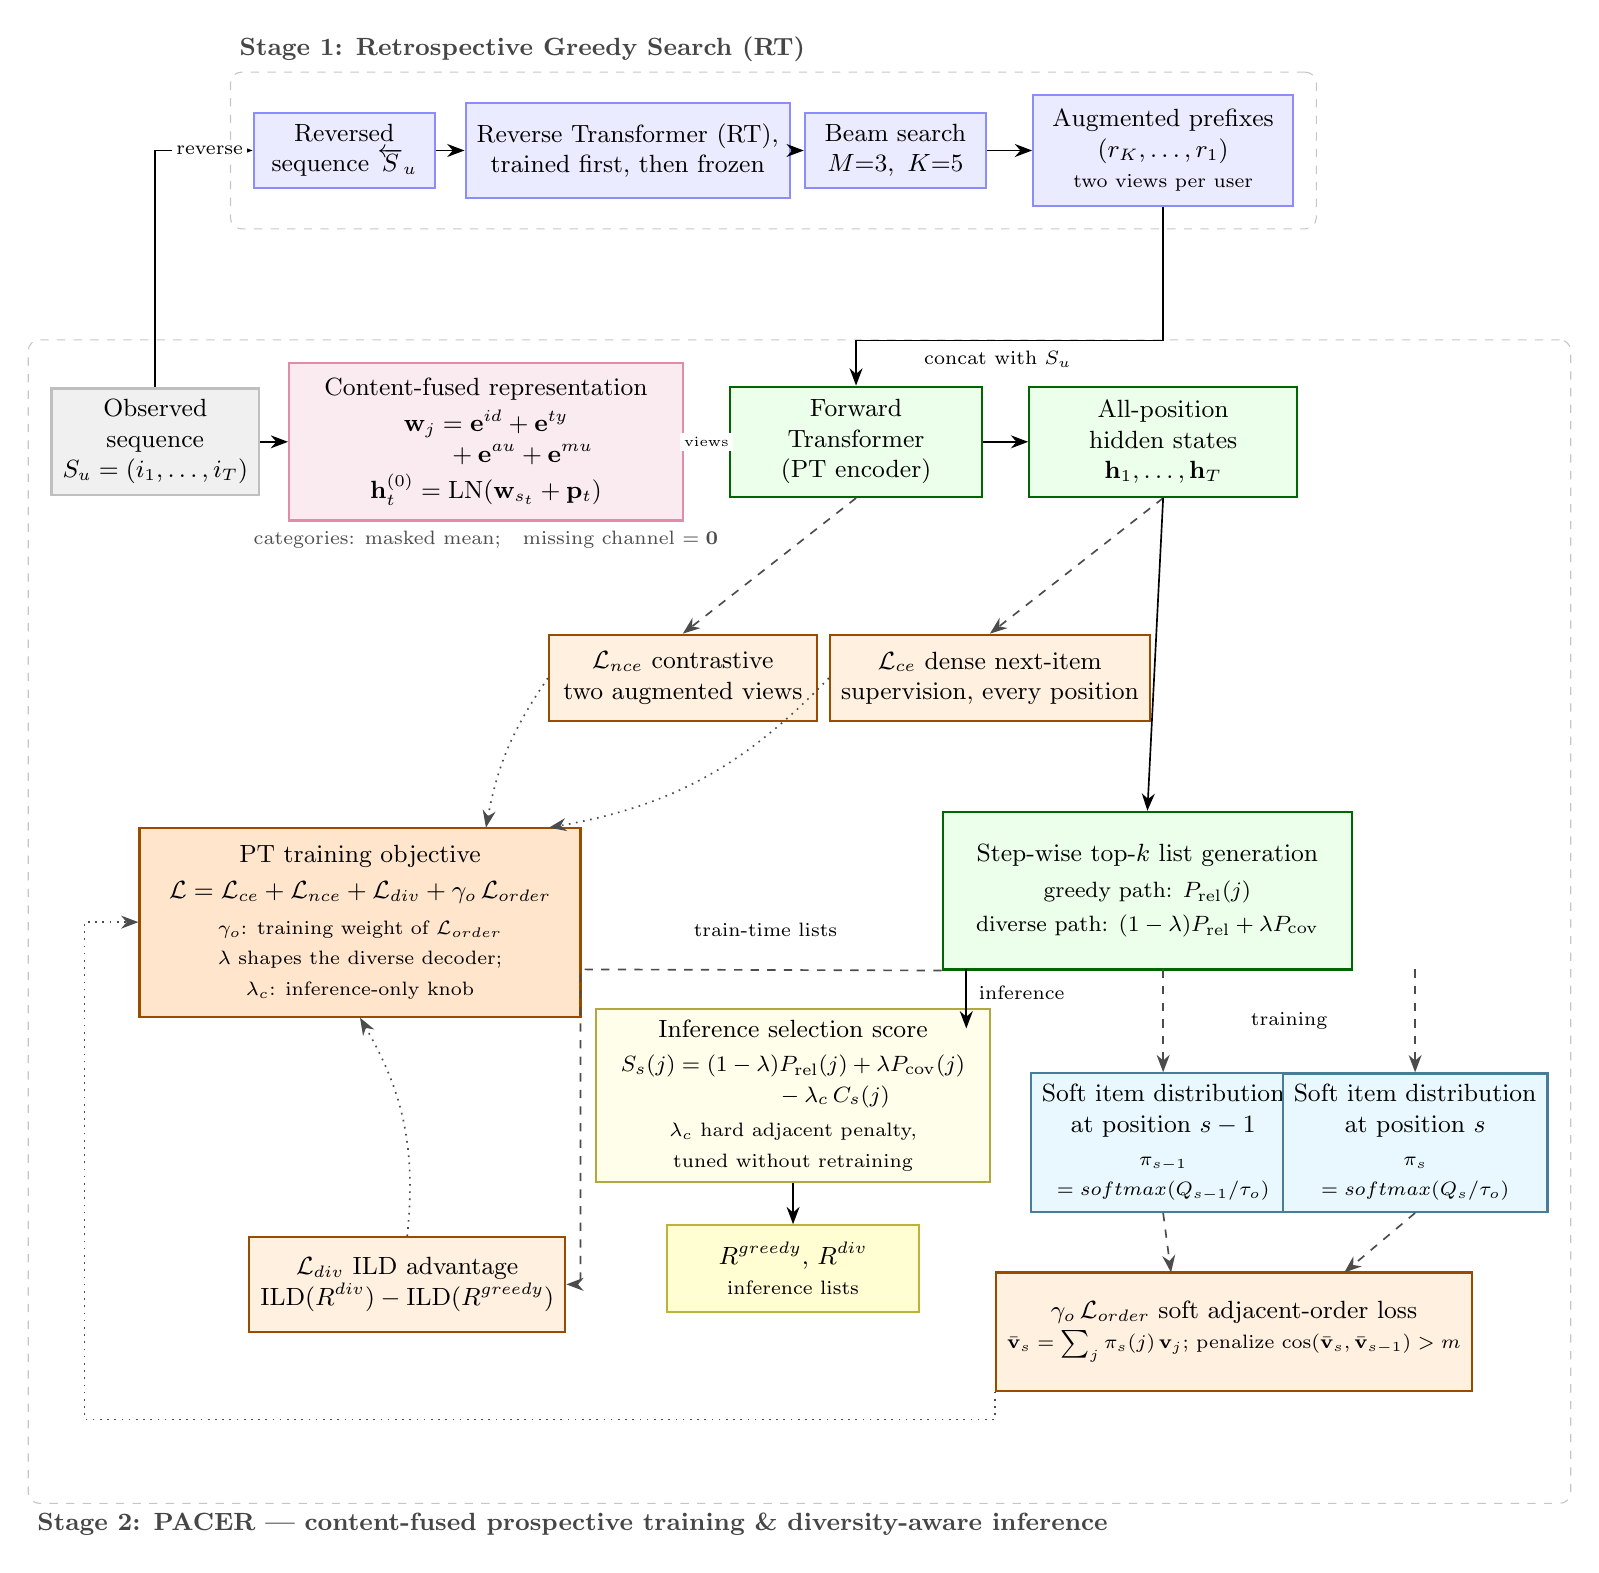
\begin{tikzpicture}[
  font=\small,
  box/.style={draw, align=center, inner sep=4pt,
              minimum height=0.95cm, thick},
  data/.style={box, fill=gray!12, draw=gray!50},
  rtb/.style={box, fill=blue!8, draw=blue!45},
  ptb/.style={box, fill=green!8, draw=green!40!black},
  emb/.style={box, fill=purple!8, draw=purple!45},
  loss/.style={box, fill=orange!12, draw=orange!60!black},
  softd/.style={box, fill=cyan!9, draw=cyan!55!black},
  lst/.style={box, fill=yellow!18, draw=yellow!70!black},
  scb/.style={box, fill=yellow!8, draw=yellow!65!black},
  arr/.style={-{Stealth[length=2.2mm]}, semithick},
  darr/.style={arr, dashed, gray!60!black},
  lbl/.style={font=\scriptsize, fill=white, inner sep=1.5pt},
  note/.style={font=\scriptsize, text=gray!60!black, align=center},
  stage/.style={draw=gray!45, dashed, rounded corners=4pt, inner sep=8pt},
  stagelbl/.style={font=\small\bfseries, text=gray!55!black}
]

% ---------------- main forward pipeline (y = 3.5) ----------------
\node[data, minimum width=2.6cm] (seq) at (0,3.5)
  {Observed\\ sequence\\ $S_u=(i_1,\ldots,i_T)$};

\node[emb, minimum width=5.0cm, minimum height=2.0cm] (fuse) at (4.2,3.5)
  {Content-fused representation\\[2pt]
   $\mathbf w_j=\mathbf e^{id}+\mathbf e^{ty}$\\
   $\phantom{\mathbf w_j=}\ +\mathbf e^{au}+\mathbf e^{mu}$\\[1pt]
   $\mathbf h_t^{(0)}=\mathrm{LN}(\mathbf w_{s_t}+\mathbf p_t)$};
\node[note, anchor=north] (fusenote) at (fuse.south)
  {categories: masked mean;\quad missing channel $=\mathbf 0$};

\node[ptb, minimum width=3.2cm, minimum height=1.4cm] (pte) at (8.9,3.5)
  {Forward\\ Transformer\\ (PT encoder)};

\node[ptb, minimum width=3.4cm, minimum height=1.4cm] (hs) at (12.8,3.5)
  {All-position\\ hidden states\\ $\mathbf h_1,\ldots,\mathbf h_T$};

\draw[arr] (seq.east) -- (fuse.west);
\draw[arr] (fuse.east) -- node[lbl, font=\tiny]{views} (pte.west);
\draw[arr] (pte.east) -- (hs.west);

% ---------------- Stage 1: RT (y = 7.2) ----------------
\node[rtb, minimum width=2.3cm] (rev) at (2.4,7.2)
  {Reversed\\ sequence $\overleftarrow S_u$};
\node[rtb, minimum width=3.2cm, minimum height=1.2cm] (rte) at (6.0,7.2)
  {Reverse Transformer (RT),\\ trained first, then frozen};
\node[rtb, minimum width=2.3cm] (beam) at (9.4,7.2)
  {Beam search\\ $M{=}3,\ K{=}5$};
\node[rtb, minimum width=3.3cm, minimum height=1.4cm] (pref) at (12.8,7.2)
  {Augmented prefixes\\ $(r_K,\ldots,r_1)$\\ {\scriptsize two views per user}};

\draw[arr] (seq.north) |- node[lbl, pos=0.78]{reverse} (rev.west);
\draw[arr] (rev.east) -- (rte.west);
\draw[arr] (rte.east) -- (beam.west);
\draw[arr] (beam.east) -- (pref.west);
% Route around the hidden-states box: down into the inter-row gap, then left,
% then into the top of the PT encoder.
\draw[arr] (pref.south) -- ++(0,-1.7) -| (pte.north);
\node[lbl] at (10.7,4.55) {concat with $S_u$};

% ---------------- training losses (y = 0.5) ----------------
\node[loss, minimum width=3.4cm, minimum height=1.1cm] (lnce) at (6.7,0.5)
  {$\mathcal L_{nce}$ contrastive\\ two augmented views};
\node[loss, minimum width=3.4cm, minimum height=1.1cm] (lce) at (10.6,0.5)
  {$\mathcal L_{ce}$ dense next-item\\ supervision, every position};
\draw[darr] (pte.south) -- (lnce.north);
\draw[darr] (hs.south) -- (lce.north);

% ---------------- total objective (bottom left) ----------------
\node[loss, fill=orange!20, minimum width=5.6cm, minimum height=2.4cm] (ltot)
  at (2.6,-2.6)
  {PT training objective\\[2pt]
   $\mathcal L=\mathcal L_{ce}+\mathcal L_{nce}+\mathcal L_{div}
    +\gamma_o\,\mathcal L_{order}$\\[2pt]
   {\scriptsize $\gamma_o$: training weight of $\mathcal L_{order}$}\\
   {\scriptsize $\lambda$ shapes the diverse decoder;}\\
   {\scriptsize $\lambda_c$: inference-only knob}};
% Both per-step losses feed the objective across its TOP edge, at distinct
% points, keeping the thin corridor UNDER the box (y=-3.2) completely clear.
\draw[darr, dotted] (lnce.west) to[bend right=12] (4.2,-1.4);
\draw[darr, dotted] (lce.west)  to[bend left=18]  (5.0,-1.4);

% ---------------- step-wise generation (right, y = -2.2) ----------------
% TRAINING-time generation: relevance path + diversity coverage path only.
% The hard adjacent penalty -lambda_c C_s(j) does NOT live here; it is applied
% exclusively in the inference selection-score node on the solid branch.
\node[ptb, minimum width=5.2cm, minimum height=2.0cm] (gen) at (12.6,-2.2)
  {Step-wise top-$k$ list generation\\[2pt]
   {\footnotesize greedy path: $P_{\mathrm{rel}}(j)$}\\[1pt]
   {\footnotesize diverse path:
    $(1-\lambda)P_{\mathrm{rel}}+\lambda P_{\mathrm{cov}}$}};
\draw[arr] (hs.south) -- (gen.north);

% ---------------- INFERENCE branch (SOLID): score then lists ---------------
% The FULL selection score, including -lambda_c C_s(j), exists only here.
\node[scb, minimum width=5.0cm, minimum height=1.7cm] (sco) at (8.1,-4.8)
  {Inference selection score\\[1.5pt]
   {\footnotesize $S_s(j)=(1-\lambda)P_{\mathrm{rel}}(j)
                       +\lambda P_{\mathrm{cov}}(j)$}\\
   {\footnotesize $\phantom{S_s(j)=}-\lambda_c\,C_s(j)$}\\[1.5pt]
   {\scriptsize $\lambda_c$ hard adjacent penalty,}\\
   {\scriptsize tuned without retraining}};
% Pure deployment output: this node has NO arrows into training losses.
\node[lst, minimum width=3.2cm, minimum height=1.1cm] (ri) at (8.1,-7.0)
  {$R^{greedy},\,R^{div}$\\ {\scriptsize inference lists}};
% Solid inference branch leaves gen just inside its SW corner and drops into
% the score node's north edge (short, entirely to the right of the score box).
\draw[arr] (10.3,-3.2) -- (10.3,-3.95);
\node[lbl, anchor=west] at (10.4,-3.5) {inference};
\draw[arr] (sco.south) -- (ri.north);

% ---------------- training-time soft distributions (DASHED branch) ----------
% The decoder scores Q_s at two adjacent positions are turned into soft item
% distributions; L_order reads BOTH of them (never an argmax'd token).
\node[softd, minimum width=3.0cm, minimum height=1.5cm] (pip) at (12.8,-5.4)
  {Soft item distribution\\ at position $s-1$\\[1pt]
   {\scriptsize $\boldsymbol\pi_{s-1}$}\\
   {\scriptsize $=\operatorname{softmax}(Q_{s-1}/\tau_o)$}};
\node[softd, minimum width=3.0cm, minimum height=1.5cm] (pi) at (16.0,-5.4)
  {Soft item distribution\\ at position $s$\\[1pt]
   {\scriptsize $\boldsymbol\pi_s$}\\
   {\scriptsize $=\operatorname{softmax}(Q_s/\tau_o)$}};
\draw[darr] (12.8,-3.2) -- (pip.north);
\draw[darr] (16.0,-3.2) -- (pi.north);
\node[lbl] at (14.4,-3.85) {training};

% ---------------- list-level training losses (bottom row) ------------------
\node[loss, minimum width=4.0cm, minimum height=1.2cm] (ldiv) at (3.2,-7.2)
  {$\mathcal L_{div}$ ILD advantage\\
   $\mathrm{ILD}(R^{div})-\mathrm{ILD}(R^{greedy})$};
\node[loss, minimum width=4.4cm, minimum height=1.5cm] (lo) at (13.7,-7.8)
  {$\gamma_o\,\mathcal L_{order}$ soft adjacent-order loss\\
   {\scriptsize $\bar{\mathbf v}_s=\sum_j \pi_s(j)\,\mathbf v_j$;
    penalize $\cos(\bar{\mathbf v}_s,\bar{\mathbf v}_{s-1})>m$}};

% Train-time list comparison: dashed, leaves the gen SW corner (the solid
% inference arrow leaves 0.3cm to its right), runs west through the clear
% corridor between objective (south -3.8) and score (north -3.95), drops in
% the gap between them, and enters L_div from the east.
\draw[darr] (gen.south west) -- (5.4,-3.2) -- (5.4,-7.2) -- (ldiv.east);
\node[lbl, anchor=north] at (7.75,-2.55) {train-time lists};

% The TWO ADJACENT SOFT DISTRIBUTIONS both point to L_order.
\draw[darr] (pip.south) -- (12.9,-7.05);
\draw[darr] (pi.south)  -- (15.1,-7.05);

% Losses roll up into the total training objective. L_div -> objective is a
% short curve on the left; L_order leaves from its SW corner along the BOTTOM
% corridor (below the inference lists and every loss box), rises in the
% far-left gap and enters the objective from the west.
\draw[darr, dotted] (ldiv.north) to[bend right=18] (ltot.south);
\draw[darr, dotted] (lo.south west) -- ++(0,-0.35) -| (-0.9,-2.6)
  -- (ltot.west);

% ---------------- stage frames ----------------
% pads keep the bottom/left L_order -> objective connector inside the frame.
\coordinate (framepad) at (8.5,-9.7);
\coordinate (framepadl) at (-1.1,-2.6);
\begin{scope}[on background layer]
  \node[stage, fit=(rev)(rte)(beam)(pref)] (st1) {};
  \node[stage, fit=(seq)(fuse)(fusenote)(pte)(hs)(lnce)(lce)(gen)
                       (sco)(ri)(pip)(pi)(ldiv)(lo)(ltot)
                       (framepad)(framepadl)] (st2) {};
\end{scope}
\node[stagelbl, anchor=south west] at (st1.north west)
  {Stage 1: Retrospective Greedy Search (RT)};
\node[stagelbl, anchor=north west] at (st2.south west)
  {Stage 2: PACER --- content-fused prospective training \& diversity-aware inference};

\end{tikzpicture}%
}
\caption{Overall PACER framework. \textbf{Stage 1 (RT):} a reverse-direction
transformer, trained independently and then frozen, hallucinates items that
could have preceded the observed sequence and returns beam-search augmented
views. \textbf{Stage 2 (PACER):} each item is represented by additive fusion of
ID, category (masked-mean pooled), creator, and music embeddings together with
a positional embedding; a forward transformer is trained with dense
per-position next-item supervision ($\mathcal L_{ce}$), cross-view contrastive
learning ($\mathcal L_{nce}$), an ILD list-diversity loss
($\mathcal L_{div}$), and a differentiable \emph{soft} adjacent-order loss
($\gamma_o\mathcal L_{order}$) computed from the soft item distributions at two
neighbouring list positions rather than from argmax tokens (solid arrows mark
the inference branch, dashed arrows the training branch). At inference, lists
are generated step by step with the combined relevance--coverage score that
additionally carries the hard adjacent-content penalty $-\lambda_c C_s(j)$;
$\lambda_c$ is tuned without retraining.}
\label{fig:pacer_framework}
\end{figure*}
.
% =============================================================================
\usetikzlibrary{arrows.meta,positioning,fit,backgrounds}

% Float placement notes (two-column):
%  - [t!] overrides LaTeX's aesthetic limits so the spanning float can take
%    the top of the *next* page even when tall.
%  - Preamble (main .tex), recommended:
%      \usepackage{dblfloatfix}                 % allow current-page placement
%      \usepackage{placeins}                    % \FloatBarrier support
%      \renewcommand{\dbltopfraction}{0.95}
%      \renewcommand{\dblfloatpagefraction}{0.7}
%  - To stop it drifting past a section, put \FloatBarrier where it must be
%    printed by (e.g. right before the next \subsection).
%  - Exact "on this page, right here" needs a non-float: use the strip
%    environment of the cuted package instead of figure*.
\begin{figure*}[t!]
\centering
% Overall size knob: fraction of the (two-column-spanning) \textwidth.
%   1.0\textwidth = full span (current); 0.8/0.7 = smaller, auto-centred.
% For a one-column figure: change figure* -> figure and use \columnwidth here.
% Prefer 0.85-1.0: below ~0.7 the scaled math/labels get hard to read; in that
% case shrink internals instead (font=\footnotesize, smaller node dimensions).
\resizebox{0.9\textwidth}{!}{%
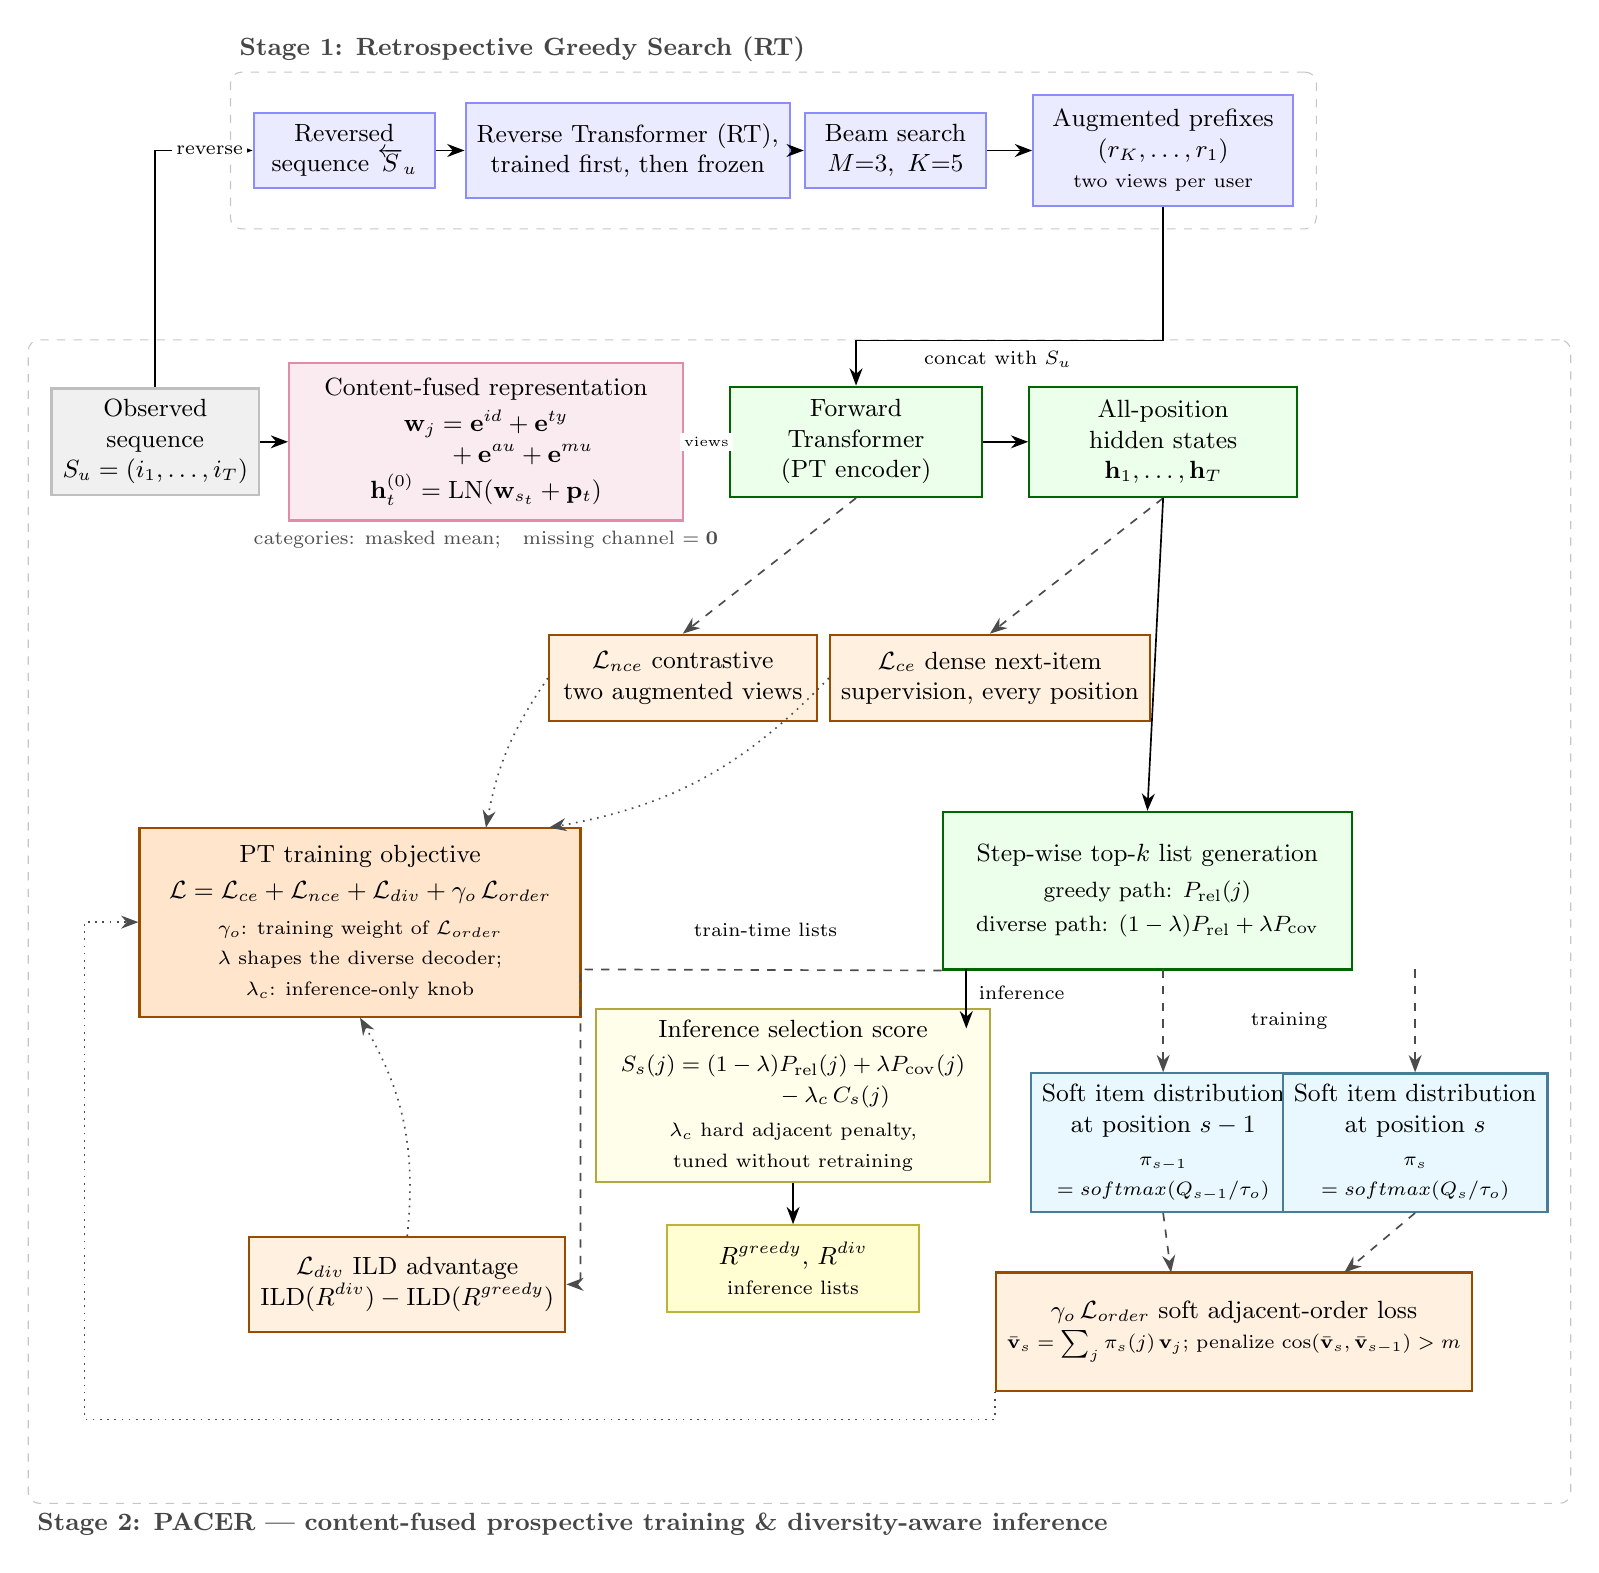
\begin{tikzpicture}[
  font=\small,
  box/.style={draw, align=center, inner sep=4pt,
              minimum height=0.95cm, thick},
  data/.style={box, fill=gray!12, draw=gray!50},
  rtb/.style={box, fill=blue!8, draw=blue!45},
  ptb/.style={box, fill=green!8, draw=green!40!black},
  emb/.style={box, fill=purple!8, draw=purple!45},
  loss/.style={box, fill=orange!12, draw=orange!60!black},
  softd/.style={box, fill=cyan!9, draw=cyan!55!black},
  lst/.style={box, fill=yellow!18, draw=yellow!70!black},
  scb/.style={box, fill=yellow!8, draw=yellow!65!black},
  arr/.style={-{Stealth[length=2.2mm]}, semithick},
  darr/.style={arr, dashed, gray!60!black},
  lbl/.style={font=\scriptsize, fill=white, inner sep=1.5pt},
  note/.style={font=\scriptsize, text=gray!60!black, align=center},
  stage/.style={draw=gray!45, dashed, rounded corners=4pt, inner sep=8pt},
  stagelbl/.style={font=\small\bfseries, text=gray!55!black}
]

% ---------------- main forward pipeline (y = 3.5) ----------------
\node[data, minimum width=2.6cm] (seq) at (0,3.5)
  {Observed\\ sequence\\ $S_u=(i_1,\ldots,i_T)$};

\node[emb, minimum width=5.0cm, minimum height=2.0cm] (fuse) at (4.2,3.5)
  {Content-fused representation\\[2pt]
   $\mathbf w_j=\mathbf e^{id}+\mathbf e^{ty}$\\
   $\phantom{\mathbf w_j=}\ +\mathbf e^{au}+\mathbf e^{mu}$\\[1pt]
   $\mathbf h_t^{(0)}=\mathrm{LN}(\mathbf w_{s_t}+\mathbf p_t)$};
\node[note, anchor=north] (fusenote) at (fuse.south)
  {categories: masked mean;\quad missing channel $=\mathbf 0$};

\node[ptb, minimum width=3.2cm, minimum height=1.4cm] (pte) at (8.9,3.5)
  {Forward\\ Transformer\\ (PT encoder)};

\node[ptb, minimum width=3.4cm, minimum height=1.4cm] (hs) at (12.8,3.5)
  {All-position\\ hidden states\\ $\mathbf h_1,\ldots,\mathbf h_T$};

\draw[arr] (seq.east) -- (fuse.west);
\draw[arr] (fuse.east) -- node[lbl, font=\tiny]{views} (pte.west);
\draw[arr] (pte.east) -- (hs.west);

% ---------------- Stage 1: RT (y = 7.2) ----------------
\node[rtb, minimum width=2.3cm] (rev) at (2.4,7.2)
  {Reversed\\ sequence $\overleftarrow S_u$};
\node[rtb, minimum width=3.2cm, minimum height=1.2cm] (rte) at (6.0,7.2)
  {Reverse Transformer (RT),\\ trained first, then frozen};
\node[rtb, minimum width=2.3cm] (beam) at (9.4,7.2)
  {Beam search\\ $M{=}3,\ K{=}5$};
\node[rtb, minimum width=3.3cm, minimum height=1.4cm] (pref) at (12.8,7.2)
  {Augmented prefixes\\ $(r_K,\ldots,r_1)$\\ {\scriptsize two views per user}};

\draw[arr] (seq.north) |- node[lbl, pos=0.78]{reverse} (rev.west);
\draw[arr] (rev.east) -- (rte.west);
\draw[arr] (rte.east) -- (beam.west);
\draw[arr] (beam.east) -- (pref.west);
% Route around the hidden-states box: down into the inter-row gap, then left,
% then into the top of the PT encoder.
\draw[arr] (pref.south) -- ++(0,-1.7) -| (pte.north);
\node[lbl] at (10.7,4.55) {concat with $S_u$};

% ---------------- training losses (y = 0.5) ----------------
\node[loss, minimum width=3.4cm, minimum height=1.1cm] (lnce) at (6.7,0.5)
  {$\mathcal L_{nce}$ contrastive\\ two augmented views};
\node[loss, minimum width=3.4cm, minimum height=1.1cm] (lce) at (10.6,0.5)
  {$\mathcal L_{ce}$ dense next-item\\ supervision, every position};
\draw[darr] (pte.south) -- (lnce.north);
\draw[darr] (hs.south) -- (lce.north);

% ---------------- total objective (bottom left) ----------------
\node[loss, fill=orange!20, minimum width=5.6cm, minimum height=2.4cm] (ltot)
  at (2.6,-2.6)
  {PT training objective\\[2pt]
   $\mathcal L=\mathcal L_{ce}+\mathcal L_{nce}+\mathcal L_{div}
    +\gamma_o\,\mathcal L_{order}$\\[2pt]
   {\scriptsize $\gamma_o$: training weight of $\mathcal L_{order}$}\\
   {\scriptsize $\lambda$ shapes the diverse decoder;}\\
   {\scriptsize $\lambda_c$: inference-only knob}};
% Both per-step losses feed the objective across its TOP edge, at distinct
% points, keeping the thin corridor UNDER the box (y=-3.2) completely clear.
\draw[darr, dotted] (lnce.west) to[bend right=12] (4.2,-1.4);
\draw[darr, dotted] (lce.west)  to[bend left=18]  (5.0,-1.4);

% ---------------- step-wise generation (right, y = -2.2) ----------------
% TRAINING-time generation: relevance path + diversity coverage path only.
% The hard adjacent penalty -lambda_c C_s(j) does NOT live here; it is applied
% exclusively in the inference selection-score node on the solid branch.
\node[ptb, minimum width=5.2cm, minimum height=2.0cm] (gen) at (12.6,-2.2)
  {Step-wise top-$k$ list generation\\[2pt]
   {\footnotesize greedy path: $P_{\mathrm{rel}}(j)$}\\[1pt]
   {\footnotesize diverse path:
    $(1-\lambda)P_{\mathrm{rel}}+\lambda P_{\mathrm{cov}}$}};
\draw[arr] (hs.south) -- (gen.north);

% ---------------- INFERENCE branch (SOLID): score then lists ---------------
% The FULL selection score, including -lambda_c C_s(j), exists only here.
\node[scb, minimum width=5.0cm, minimum height=1.7cm] (sco) at (8.1,-4.8)
  {Inference selection score\\[1.5pt]
   {\footnotesize $S_s(j)=(1-\lambda)P_{\mathrm{rel}}(j)
                       +\lambda P_{\mathrm{cov}}(j)$}\\
   {\footnotesize $\phantom{S_s(j)=}-\lambda_c\,C_s(j)$}\\[1.5pt]
   {\scriptsize $\lambda_c$ hard adjacent penalty,}\\
   {\scriptsize tuned without retraining}};
% Pure deployment output: this node has NO arrows into training losses.
\node[lst, minimum width=3.2cm, minimum height=1.1cm] (ri) at (8.1,-7.0)
  {$R^{greedy},\,R^{div}$\\ {\scriptsize inference lists}};
% Solid inference branch leaves gen just inside its SW corner and drops into
% the score node's north edge (short, entirely to the right of the score box).
\draw[arr] (10.3,-3.2) -- (10.3,-3.95);
\node[lbl, anchor=west] at (10.4,-3.5) {inference};
\draw[arr] (sco.south) -- (ri.north);

% ---------------- training-time soft distributions (DASHED branch) ----------
% The decoder scores Q_s at two adjacent positions are turned into soft item
% distributions; L_order reads BOTH of them (never an argmax'd token).
\node[softd, minimum width=3.0cm, minimum height=1.5cm] (pip) at (12.8,-5.4)
  {Soft item distribution\\ at position $s-1$\\[1pt]
   {\scriptsize $\boldsymbol\pi_{s-1}$}\\
   {\scriptsize $=\operatorname{softmax}(Q_{s-1}/\tau_o)$}};
\node[softd, minimum width=3.0cm, minimum height=1.5cm] (pi) at (16.0,-5.4)
  {Soft item distribution\\ at position $s$\\[1pt]
   {\scriptsize $\boldsymbol\pi_s$}\\
   {\scriptsize $=\operatorname{softmax}(Q_s/\tau_o)$}};
\draw[darr] (12.8,-3.2) -- (pip.north);
\draw[darr] (16.0,-3.2) -- (pi.north);
\node[lbl] at (14.4,-3.85) {training};

% ---------------- list-level training losses (bottom row) ------------------
\node[loss, minimum width=4.0cm, minimum height=1.2cm] (ldiv) at (3.2,-7.2)
  {$\mathcal L_{div}$ ILD advantage\\
   $\mathrm{ILD}(R^{div})-\mathrm{ILD}(R^{greedy})$};
\node[loss, minimum width=4.4cm, minimum height=1.5cm] (lo) at (13.7,-7.8)
  {$\gamma_o\,\mathcal L_{order}$ soft adjacent-order loss\\
   {\scriptsize $\bar{\mathbf v}_s=\sum_j \pi_s(j)\,\mathbf v_j$;
    penalize $\cos(\bar{\mathbf v}_s,\bar{\mathbf v}_{s-1})>m$}};

% Train-time list comparison: dashed, leaves the gen SW corner (the solid
% inference arrow leaves 0.3cm to its right), runs west through the clear
% corridor between objective (south -3.8) and score (north -3.95), drops in
% the gap between them, and enters L_div from the east.
\draw[darr] (gen.south west) -- (5.4,-3.2) -- (5.4,-7.2) -- (ldiv.east);
\node[lbl, anchor=north] at (7.75,-2.55) {train-time lists};

% The TWO ADJACENT SOFT DISTRIBUTIONS both point to L_order.
\draw[darr] (pip.south) -- (12.9,-7.05);
\draw[darr] (pi.south)  -- (15.1,-7.05);

% Losses roll up into the total training objective. L_div -> objective is a
% short curve on the left; L_order leaves from its SW corner along the BOTTOM
% corridor (below the inference lists and every loss box), rises in the
% far-left gap and enters the objective from the west.
\draw[darr, dotted] (ldiv.north) to[bend right=18] (ltot.south);
\draw[darr, dotted] (lo.south west) -- ++(0,-0.35) -| (-0.9,-2.6)
  -- (ltot.west);

% ---------------- stage frames ----------------
% pads keep the bottom/left L_order -> objective connector inside the frame.
\coordinate (framepad) at (8.5,-9.7);
\coordinate (framepadl) at (-1.1,-2.6);
\begin{scope}[on background layer]
  \node[stage, fit=(rev)(rte)(beam)(pref)] (st1) {};
  \node[stage, fit=(seq)(fuse)(fusenote)(pte)(hs)(lnce)(lce)(gen)
                       (sco)(ri)(pip)(pi)(ldiv)(lo)(ltot)
                       (framepad)(framepadl)] (st2) {};
\end{scope}
\node[stagelbl, anchor=south west] at (st1.north west)
  {Stage 1: Retrospective Greedy Search (RT)};
\node[stagelbl, anchor=north west] at (st2.south west)
  {Stage 2: PACER --- content-fused prospective training \& diversity-aware inference};

\end{tikzpicture}%
}
\caption{Overall PACER framework. \textbf{Stage 1 (RT):} a reverse-direction
transformer, trained independently and then frozen, hallucinates items that
could have preceded the observed sequence and returns beam-search augmented
views. \textbf{Stage 2 (PACER):} each item is represented by additive fusion of
ID, category (masked-mean pooled), creator, and music embeddings together with
a positional embedding; a forward transformer is trained with dense
per-position next-item supervision ($\mathcal L_{ce}$), cross-view contrastive
learning ($\mathcal L_{nce}$), an ILD list-diversity loss
($\mathcal L_{div}$), and a differentiable \emph{soft} adjacent-order loss
($\gamma_o\mathcal L_{order}$) computed from the soft item distributions at two
neighbouring list positions rather than from argmax tokens (solid arrows mark
the inference branch, dashed arrows the training branch). At inference, lists
are generated step by step with the combined relevance--coverage score that
additionally carries the hard adjacent-content penalty $-\lambda_c C_s(j)$;
$\lambda_c$ is tuned without retraining.}
\label{fig:pacer_framework}
\end{figure*}
